\documentclass[11pt]{article}
\usepackage{latexsym}
\usepackage{amsmath}
\usepackage{amssymb}
\usepackage{amsthm}
\usepackage{epsfig}
\usepackage{graphicx}
\usepackage[tight]{subfigure}
% \usepackage{subcaption}
\usepackage{hyperref}

\usepackage{amsmath}
\usepackage{mathrsfs}
\usepackage{bbm}

\DeclareMathOperator*{\minimize}{min}
\DeclareMathOperator*{\maximize}{max}
\DeclareMathOperator*{\argmax}{arg\,max}
\DeclareMathOperator*{\argmin}{arg\,min}

\def\RR{\mathbb{R}}
\def\BB{\mathbb{B}}
\def\AA{\mathbb{A}}
\def\PP{\mathbb{P}}
\def\EE{\mathbb{E}}
\def\FF{\mathbb{F}}
\def\HH{\mathcal{H}}
\def\XX{\mathcal{X}}
\def\YY{\mathcal{Y}}
\def\NN{\mathbb{N}}
\def\TT{\mathcal{T}}
\def\DD{\mathcal{D}}
\def\SS{\mathcal{S}}
\def\LL{\mathcal{L}}
\def\MM{\mathcal{M}}
\def\err{\text{err}}
\def\ind{\mathbbm{1}}
\def\II{\mathcal{I}}
\def\ig{\mathcal{\gemini}}
\def\Lev{\textscl}



\usepackage{algorithm}
 %on linux you may need to run sudo apt-get install texlive-full to install algorithm.sys
\usepackage{algorithmic}

\usepackage{verbatim}

\newcommand{\handout}[5]{
  \noindent
  \begin{center}
  \framebox{
    \vbox{
      \hbox to 5.78in { {#1} \hfill #2 }
      \vspace{4mm}
      \hbox to 5.78in { {\Large \hfill #5  \hfill} }
      \vspace{2mm}
      \hbox to 5.78in { {\em #3 \hfill #4} }
    }
  }
  \end{center}
  \vspace*{4mm}
}

\newcommand{\lecture}[5]{\handout{#1}{#2}{#3}{#4}{#5}}
\newcommand{\collision}[0]{\mathrm{collision}}
\newcommand{\nocollision}[0]{\overline{\collision}}

\newcommand*{\QED}{\hfill\ensuremath{\square}}

\newtheorem{theorem}{Theorem}
\newtheorem{corollary}[theorem]{Corollary}
\newtheorem{lemma}[theorem]{Lemma}
\newtheorem{observation}[theorem]{Observation}
\newtheorem{proposition}[theorem]{Proposition}
\newtheorem{definition}[theorem]{Definition}
\newtheorem{claim}[theorem]{Claim}
\newtheorem{fact}[theorem]{Fact}
\newtheorem{assumption}[theorem]{Assumption}
\newtheorem{note}[theorem]{Note}

% 1-inch margins, from fullpage.sty by H.Partl, Version 2, Dec. 15, 1988.
\topmargin 0pt
\advance \topmargin by -\headheight
\advance \topmargin by -\headsep
\textheight 8.9in
\oddsidemargin 0pt
\evensidemargin \oddsidemargin
\marginparwidth 0.5in
\textwidth 6.5in

\parindent 0in
\parskip 1.5ex
%\renewcommand{\baselinestretch}{1.25}

\begin{document}

\lecture{Statistical Techniques in Robotics (16-831, S22)}{Lecture \#19
  (Wednesday, March 30, 2022)}{Lecturer: Kris Kitani}{Scribes: Lulu Ricketts and Shane Deng}{Model Free Control and Function Approximation}

\section{Review}

% \begin{figure}[h]
% \centering
% \begin{subfigure}[t]{0.5\textwidth}
%   \centering
%   \includegraphics[width=.3\linewidth]{Hard SVM.png}
%   \caption{Hard SVM}
%   \label{fig:sfig6}
% \end{subfigure}%
% \begin{subfigure}[t]{0.5\textwidth}
%   \centering
%   \includegraphics[width=.3\linewidth]{Soft SVM.png}
%   \caption{Soft SVM}
%   \label{fig:sfig6}
% \end{subfigure}
% \end{figure}


% \begin{algorithm}[H]
% \caption{Soft SVM}
% \label{algo:SVM}
% \begin{algorithmic}[1]
% \STATE $\mathbf{w}^{(0)} \leftarrow 0 \in R^N$ \COMMENT{Written in OMD format} \hfill
% \FOR{$t=0,\;\cdots,\;T-1$}
% \STATE \textsc{Receive} ($\textbf y_d, x_d \sim D$) \COMMENT{Receive sample from environment (training data)} \hfill 
% \STATE $\pmb{\theta}^t = \pmb{\theta}^{(t-1)} + y_d x_d \cdot \mathbbm{1}[y_d(\mathbf{w}^{(t)} \mathbf{x}_d) < 1]$ \COMMENT{Dual parameter update} \hfill
% \STATE $\mathbf{w}^{(t+1)}\leftarrow \dfrac{1}{\lambda (t+1)} \pmb{\theta}^t$ \COMMENT{Mirror projection} \hfill
% \ENDFOR
% \end{algorithmic}
% \end{algorithm}

\subsection{Reinforcement Learning Big Picture}

So far in our coverage of reinforcement learning algorithms, we have been focusing on tabular value-based algorithms; tabular meaning that we have a reasonably-sized finite state space such that the value function (or action-value function) can be stored and updated through the use of a table. Value-based algorithms directly estimate the value function under a policy given an environment of states and actions. 

Value-based algorithms can be further subcategorized into model-based and model-free algorithms, distinguished by how much information about the environment we have access to. Model-based algorithms are those that can access state transition dynamics and reward functions, thus are able to use the Bellman equation (\ref{eq:1}) to compute value functions without direct interaction with the environment.

\begin{align}
\label{eq:1}
    V^{\pi}(s) = \sum_a \pi(a|s)\sum_{s'}p(s'|s,a)[r(s',a,s) + \gamma V^{\pi}(s')]
\end{align}

In contrast, model free algorithms do not have access to this information, and have to update their value functions through direct interactions with the environment, which gives the next state and action, in discrete time steps.

\subsection{Model Free Methods for Prediction and Control}

\begin{figure}[H]
    \centering
    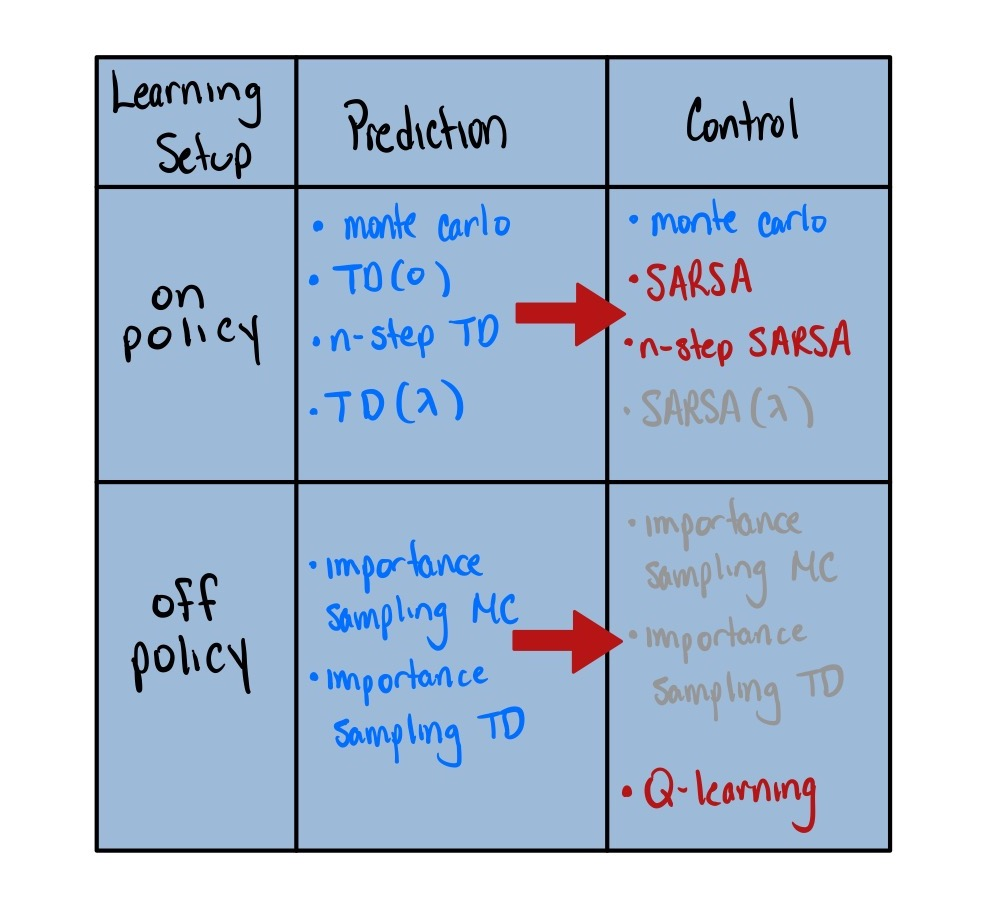
\includegraphics[scale=0.17]{images/Page1 2.jpg}
    \caption{Table of Model-Free Methods}
    \label{fig:modelfree}
\end{figure}

Table 1 shows the different learning algorithms that fall under model free reinforcement learning. These algorithms can either be prediction or control, and either on-policy or off-policy algorithms. Those in blue have been covered in previous lectures, those in red are what will be covered here, and those in gray have not been covered yet. As shown in the figure, each prediction algorithm has a corresponding control algorithm. In fact, it is very easy to transition from prediction to control by simply adding a policy improvement step to the algorithm.

\subsubsection{On Policy vs. Off Policy}

The key difference between on policy and off policy is off-policy's differentiation between the policy we follow and the policy whose value function we update. We refer to the policy we follow as the behavior policy, while the target policy is the one we care about that leads us to the optimal policy. Generally in off policy algorithms, we directly update the behavior policy and the value function of the target policy. It is not always necessary to update the behavior policy, although doing so may be helpful to accelerate learning.

In on policy algorithms, the behavior and target policies are the same, therefore both are referred to as the target policy.

There are several benefits to following an off policy algorithm:
\begin{enumerate}
    \item You can learn using experiences of other agents
    \item You can learn multiple policies using a single behavior policy
    \item You can leverage your own past experience to learn
    \item Target policies could be expensive to run in certain applications
\end{enumerate}

One important property of off policy algorithms is that they must satisfy the coverage ("full support") assumption, stating that the behavior policy $\mu(a|s)$ must visit all parts of the state space to accurately estimate the target policy:

\begin{align}
\label{eq:2}
    \text{If } \pi(a|s) > 0\text{, then it must be that }\mu(a|s) > 0
\end{align}

To satisfy this, many behavior policies follow an $\epsilon$-greedy algorithm so as to retain exploration to unseen or less explored states in the environment.

\subsubsection{Prediction vs. Control}

Another distinction under model-free RL methods is that between prediction and control. Figure \ref{fig:predvcontrol} shows the entire value-based learning loop. While in lecture they have been taught separately, control simply adds a policy improvement step to the prediction algorithm. This policy improvement is important when learning so that we not only update our value function, but also improve upon the policy which we follow.

\begin{figure}[H]
    \centering
    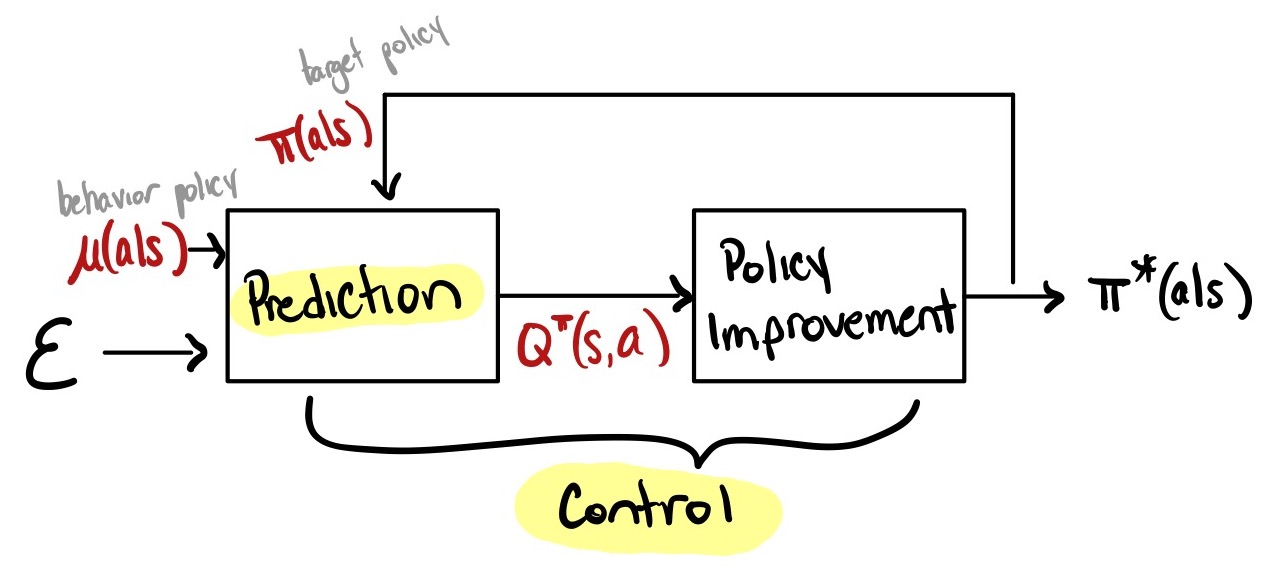
\includegraphics[width=0.7\textwidth]{images/Page2 2.jpg}
    \caption{Value-Based Model-Free RL: Prediction vs. Control}
    \label{fig:predvcontrol}
\end{figure}


\subsection{Temporal Difference Prediction}

Temporal difference, or TD, prediction was taught in a previous lecture, but gets built upon more in this lecture. As we can observe in Figure \ref{fig:modelfree}, the control version of on policy TD is called SARSA, and of off policy TD is called Q-learning, both of which will be covered in this lecture. 

\subsubsection{n-Step TD}

To best understand TD learning is to understand the n-step generalization of TD prediction. In TD prediction, the value function update step follows the same structure as the Monte Carlo update, namely:

\begin{align}
\label{eq:3}
    V(s^t) \leftarrow V(s^t) + \alpha (G^t - V(s^t))
\end{align}

However, where in Monte Carlo $G^t$ is the (discounted) sum over all future rewards, the value of the return $G^t$ in the TD update equation is the (discounted) sum over the next $N-1$ rewards, and uses bootstrapping for rewards $N$ and beyond. Bootstrapping here indicates that the rewards where $t > N$ is represented by the value function's estimate at state $t+N$:

\begin{align}
\label{eq:4}
    G^t(N) = r^t + \gamma r^{t+1} + \dots + \gamma^{N-1}r^{N-1} + \gamma^NV(s^{t+N})
\end{align}

For 1-step TD (also known as TD(0)), the entire update equation is as follows, where the difference that is multiplied by $\alpha$ is known as the TD error:

\begin{align}
\label{eq:5}
    V(s^t) \leftarrow V(s^t) + \alpha (r^t + \gamma V(s^{t+1}) - V(s^t))
\end{align}



\section{SARSA}

Now that we have reviewed value-based model-free prediction, we can get into the control versions of these algorithms (mostly of TD). The first is called SARSA, which is also commonly known as "on policy 1-step TD control" or "modified connectionist q-learning" (from the original 1994 paper). 

The name SARSA comes from the fact that we use the current state and action (S,A), to get the next reward, next state, and next action simultaneously from the environment (R,S,A), which we can see in line 4 of the algorithm below.


\begin{algorithm}[H]
\caption{SARSA (on policy TD control)}
\label{algo:Sarsa}
\begin{algorithmic}[1]
\FOR{$e=0,\;\cdots,\;E$}
\STATE $\{s^{(0)},a^{(0)}\} \sim \mathcal{E}|\pi$ \hfill
\FOR{$t=0,\;\cdots,\;T$}
\STATE $\{s^{(t)},a^{(t)},r^{(t)},s^{(t+1)},a^{(t+1)}\} \sim \mathcal{E}|\pi, s^{(t)},a^{(t)}$ \hfill
\STATE $G^{(t)} = r^{(t)} + \gamma Q(a^{(t+1)},x^{(t+1)})$ \COMMENT{TD prediction}
\STATE $Q(a^{(t)},s^{(t)}) \leftarrow Q(a^{(t)},s^{(t)}) + \alpha[G^{(t)} - Q(a^{(t)},s^{(t)})]$ \hfill
\STATE $\pi(a|s) \leftarrow \frac{\epsilon}{|\mathcal{A}|} + \ind{[a = \text{argmax}_i Q(i,s)]} (1 - \epsilon) \forall{a,s}$ \COMMENT{policy improvement} \hfill
\ENDFOR
\ENDFOR
\STATE \textbf{return} $\pi^*$ \hfill
\end{algorithmic}
\end{algorithm}

This algorithm is almost exactly the same as that of TD(0) prediction, with an extra policy improvement step in line 7, which updates the policy in order to return the optimal policy $\pi^*$ in line 10. During this policy improvement, we also have a hyperparameter $\epsilon$, which denotes our $\epsilon$-soft policy to retain exploration (satisfying the coverage assumption).

There are a couple benefits to extending the TD(0) algorithm to the control case, including:
\begin{enumerate}
    \item Improves the policy we follow
    \item Can evaluate using incomplete sequences because of online updates
    \item Lower variance in policy predictions
    \item None of the TD Prediction benefits are lost (including outperforming MC prediction/control)
\end{enumerate}


\section{Q-learning}

Now that we have gone over SARSA, the on-policy control version of TD Learning, we will look at Q-Learning, also known as "off policy 1-step TD control". As the name implies, it is an off policy control algorithm that uses 1-step TD updates to get the value for the return.

\begin{algorithm}[H]
\caption{Q-Learning (off policy TD control)}
\label{algo:Q}
\begin{algorithmic}[1]
\FOR{$e=0,\;\cdots,\;E$}
\STATE $s^{(0)} \sim \mathcal{E}|\mu$ \COMMENT{sample from behavior policy}\hfill
\FOR{$t=0,\;\cdots,\;T$}
\STATE $\{s^{(t)},a^{(t)},r^{(t)},s^{(t+1)}\} \sim \mathcal{E}|\mu, s^{(t)}$ \hfill
\STATE $a^{*(t)} \leftarrow \pi(s^{(t+1)}) \triangleq \text{argmax}_a Q(a,s^{(t+1)})$ \COMMENT{greedy target policy}\hfill
\STATE $G^{(t)} = r^{(t)} + \gamma Q^{\pi}(a^{*(t)},s^{(t+1)})$ \COMMENT{TD prediction}
\STATE $Q^{\pi}(a^{(t)},s^{(t)}) \leftarrow Q^{\pi}(a^{(t)},s^{(t)}) + \alpha[G^{(t)} - Q^{\pi}(a^{(t)},s^{(t)})]$ \hfill
\STATE $\mu(a|s^{(t+1)}) \leftarrow \frac{\epsilon}{|\mathcal{A}|} + \ind{[a = \pi(s^{(t+1)})]} (1 - \epsilon) \forall{a}$ \COMMENT{policy improvement} \hfill
\ENDFOR
\ENDFOR
\STATE \textbf{return} $Q^{\pi*}$,$\pi^*$ \hfill
\end{algorithmic}
\end{algorithm}

Because Q-learning is an off-policy learning algorithm, our states and actions come from sampling our behavior policy $\mu(a|s)$ in order to get the next reward and next state. This is observable in lines 2, 4, and 8, the latter where we update the behavior policy (as opposed to the target policy in on-policy methods). There are again many similarities to both the TD(0) and SARSA algorithms here, including TD prediction steps in lines 6/7 and $\epsilon$-greedy behavior policies for exploration.

One key difference that arises from off-policy control in Q-learning is line 5. Here we receive the target action $a^{*(t)}$ that would have been chosen by the \textbf{greedy} target policy. The algorithm uses this action's associated value function to calculate the return based off this action. Thus, the TD error here (in line 7) can be thought of as the difference between $G^{(t)}$, what the target policy would have gotten as a reward following $a^{*(t)}$, and $Q^{\pi}$ following the action $a^{(t)}$ that the behavior policy had chosen to take.



\section{Non-tabular RL}

Previously we were looking at tabular RL algorithms, where our value/action-value functions are stored in a table that we continuously update as we progress through episodes of learning. This is because up until now, our state spaces were able to be discretized such as the grid world example that we have been dealing with.\\

However this isn't really the case for most reinforcement learning applications. Now we transition to thinking about how to approximate value functions in very large or continuous state spaces. One way to solve this problem is to use a function to approximate the value function. \\

As we see \ref{fig:approximator}, in the discretized world, the mapping function essentially computes the value function with a discretized set of actions. In the continuous world, actions are continuous in a sense that we have infinite amount of potential actions.
\begin{figure}[H]
    \centering
    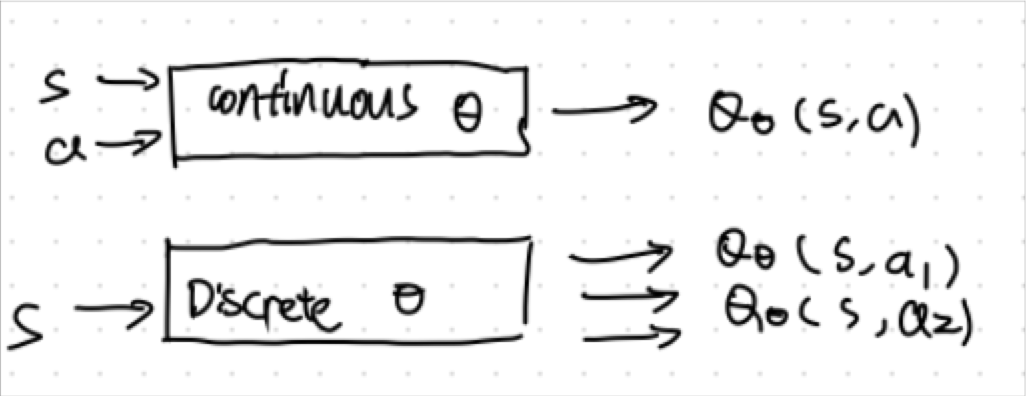
\includegraphics[width=0.7\textwidth]{images/pic1.png}
    \caption{Mapping function for both continuous and discrete worlds}
    \label{fig:approximator}
\end{figure}

\section{Value Function Approximator categories}
\begin{enumerate}
    \item Linear Approximator: \\
    $$V_\theta(s) = \theta^T f(s)$$\\
    usually, the linear approximator is just a hand-crafted matrix to scale each feature properly. This approach becomes less practical when the model is complicated
    
    \item Neural Network:\\
        $$V_\theta(s) = NN(s)$$\\
        Neural networks can be used to approximate the value function. Usually they are consisted of a feedforward single layer neural network.
        
     \item Deep Neural Network:\\
        $$V_\theta(s) = DNN(s)$$\\
        Deep neural networks are built on top of neural networks with more hidden layers so the approximated value function will be closer to the actual function
    
\end{enumerate}


\subsection{Tabular RL as function approximator}

Tabular RL is a simple (linear) function approximator where the state feature (or state-action) is an "indicator" feature. \\
$$f_d (s,a) = 1 [(s,a)=(s_d,a_d)] \; s \in S \: a \in A  $$ 
Then the value function becomes: $V(s_d,a_d) = \theta^t f(s_d,a_d) = \theta_d$. Essentially, we can plug the discretized action and state into our value function to get tabular case.

\subsection{Function approximation objective and optimization}
The goal of such approximation is: 
$V_{\theta}(s) \approx V^{\pi}(x)$ \\ since we want our approximated value function to be as close to the real value function as possible. \\
Hence the objective function can be specified as the squared difference between the approximated value function and the actual function.\\
$$\hat{\theta} = argmin_{\theta} E_p [(V(s) - V_\theta (s))^2]$$
\textbf{Note:} $E_p$ is the distribution defined by MDP \\

The objective function can be further optimized as:  $\hat{\theta} = argmin \: E_p [\dfrac{1}{2} (V(s) - V_{\theta}(s))^2 = argmin J(\theta)$\\ 

This is very similar to the online gradient descent that we have covered in the first half of the semester\\
$$\hat{\theta} = argmin_\theta \{ \alpha (J(\theta') + <\theta - \theta',\nabla_{\theta'} J(\theta')>) + \dfrac{1}{2} ||\theta - \theta' ||^2 \}$$ \\
Solve the equation by using the Lagrangian method:$$\nabla_\theta \{ \alpha (J(\theta') + <\theta - \theta',\nabla_{\theta'} J(\theta')>) + \dfrac{1}{2} ||\theta - \theta' ||^2 \}$$\\
Then solve the Lagrangian optimization:
$$\theta \leftarrow \theta' - \alpha \nabla_{\theta'} J(\theta')$$ \\

However, we will not be able to solve $\nabla_{\theta'} J(\theta')$. In order to solve the equation, we have to know the distribution $E_p$. However, in this case, we don't have direct access to this parameter since we don't roll out all possible trajectories. One way to approximate it is by using stochastic gradient descent:
$$\nabla_\theta J(\theta) \approx {(V(s) - V_\theta(s)) \dfrac{\partial}{\partial \theta}V_\theta(s)}$$
However, in this case, we still don't have direct access to the underlying true value function $V(s)$. We can use an estimate of the expected return like we did in the previous lectures:
$$V(s) = E[G^{t}] = G^{(t)}$$\\
Then we can use any of the estimated return methods like MC, TD-1 step, TD-N step and so on. 
\begin{center}
\begin{tabular}{ |c|c| } 
\hline
Method & G estimate  \\
\hline
 MC & $\sum_{i=t}^T r^i$ \\ 
 TD-1 step & $r^t + \gamma V(s^{t+1})$ \\ 
 TD-N step & $\sum_{i=t}^{t+N-1} \gamma^{i-t} r^i + \gamma^N V(s^(t+N)) $ \\ 
 $\lambda$ Return & $(1-\lambda)\sum_{n=1}^\infty \lambda^{n-1} G^t(n)$ \\ 
 TD($\lambda$) step & $z^t(s) [r^t + \gamma V(s^(t+1))]$ \\ 
 IS-MC & $\prod_{t=1}^t \dfrac{\pi(a^i | s^i)}{\mu(a^i | s^i)} \sum_{j=t}^T r^j$ \\ 
 IS-TD 1 step & $\dfrac{\pi(a^i | s^i)}{\mu(a^i | s^i)} [r^t + \gamma V(s^{t+1})]$ \\ 
\hline
\end{tabular}
\end{center}

\subsection{MC Prediction for continuous state spaces}
\begin{algorithm}[H]
\caption{Continuous MC Prediction}
\label{algo:CMC}
\begin{algorithmic}[1]
\FOR{$e=0,\;\cdots,\;E$}
\STATE $\{s^t,a^t,r^t \}_{t=0}^T \sim \mathcal{E}|\pi$
\COMMENT{sample from behavior policy}\hfill
\FOR{$t=0,\;\cdots,\;T$}
\STATE $G^t \leftarrow \sum_{i=t}^T r^t$ \hfill
\STATE $\theta \leftarrow \theta + \alpha{(G(t) - V_\theta(s^t)) \dfrac{\partial}{\partial \theta}V_\theta(s^t)}$ 
\ENDFOR
\ENDFOR
\STATE \textbf{return} $V(s)$ \hfill
\end{algorithmic}
\end{algorithm}

Recall that if it is the tabular case, we will use the indicator functions: $f_d(s) = 1[s = s_d]$ Then in line 5, the derivative with respect to the mapping function will always be 1 since it is an indicator function. Then essentially we are getting back to the tabular prediction algorithm

\subsection{MC Prediction for discretized state spaces}
\begin{algorithm}[H]
\caption{Discretized MC Prediction}
\label{algo:DMC}
\begin{algorithmic}[1]
\FOR{$e=0,\;\cdots,\;E$}
\STATE $\{s^t,a^t,r^t \}_{t=0}^T \sim \mathcal{E}|\pi$
\COMMENT{sample from behavior policy}\hfill
\FOR{$t=0,\;\cdots,\;T$}
\STATE $G^t \leftarrow \sum_{i=t}^T r^t$ \hfill
\STATE $V(s^t) \leftarrow V(s^t) + \alpha{(G(t) - V_\theta(s^t)) }$ 
\ENDFOR
\ENDFOR
\STATE \textbf{return} $V(s)$ \hfill
\end{algorithmic}
\end{algorithm}

\section{Summary}
In this lecture, we primarily focus on model free value based control algorithm. As we can see, the control algorithm is very similar to the predication algorithm just with some minor changes. We also take a look at how to approximate the value function when we don't have access to the true underlying value function in the continuous space

\section{Appendix}
\subsection{Q learning and its supplements}
As we have seen in this lecture, that Q learning is extremely useful in the off-policy situation where the state transition probabilities are not known. Compared to the previous methods that we learned like value iteration, which requires the knowledge of the transition dynamics, Q learning can essentially learn and figure out the new actions by entering a new state from its prior knowledge. \\
Although, the world is a continuous space, in the background, Q learning is essentially exploring all the possibilities and creating a Q value table. This is essentially the memory of the algorithm as we can see in algorithm 2:
$$Q^{\pi}(a^{(t)},s^{(t)}) \leftarrow Q^{\pi}(a^{(t)},s^{(t)}) + \alpha[G^{(t)} - Q^{\pi}(a^{(t)},s^{(t)})]$$ \\
However, there are some problems with this approach. 
\begin{enumerate}
    \item In a complicated world with a lot of actions and states, storing previous knowledge can take up a large amount of space.
    \item The efficiency of the algorithm will decrease because it takes longer to query the tabel and find $argmax \; Q$ 
\end{enumerate}

\subsubsection{Deep Q Networks}
This presents a possible solution to the traditional Q learning. Since we will be replacing the core of the algorithm with neural networks to approximate the Q value like we talk about previously

\begin{figure}[H]
    \centering
    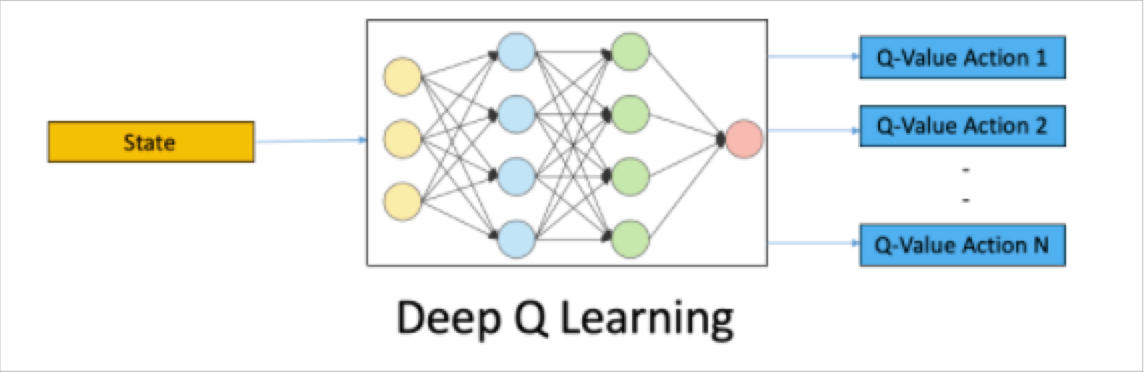
\includegraphics[width=0.7\textwidth]{images/pic2.png}
    \caption{Deep Q learning algorithm}
    \label{fig:DQN}
\end{figure}

\subsubsection{Double Q learning}
One possibly problem with our target value function in our traditional Q learning as it is shown in algorithm 2 is that we are using the greedy approach:
$$a^{*(t)} \leftarrow \pi(s^{(t+1)}) \triangleq \text{argmax}_a Q(a,s^{(t+1)})$$
As we can see, we are always taking the max estimated value. This might lead to overestimation which is called maximization bias. We are using bootstrapping technique here to estimate based on estimate. Overestimating can compound over time and could be problematic. One example is that assuming the true Q value is 0 and our estimated distribution is around 0. However, if we always take the max Q value, this will lead to the problem that we are only selecting one tail of the distribution, causing overestimation. \\
A possible solution is to use double Q learning. There are many different formulation of the double Q learning. But the key idea remains the same where we will have two separate Q value estimators and they are closely tangled together and they update based on each other. In this way, we can unbias the Q value by selecting the opposite estimator.\\
The fundamental one is shown below:
\begin{figure}[H]
    \centering
    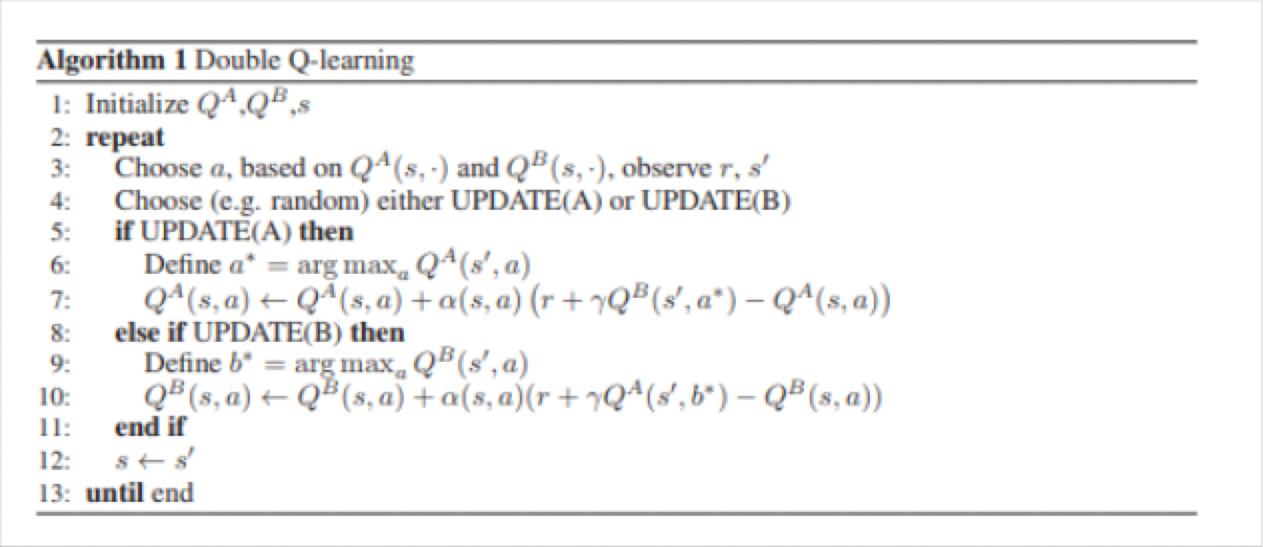
\includegraphics[width=0.7\textwidth]{images/pic3.png}
    \caption{Double Q learning algorithm}
    \label{fig:DQN}
\end{figure}

As we can see in the algorithm, we will have two different Q estimator, Qa and Qb. Then every iteration, the algorithm will randomly select which algorithm to update and use for Q value estimation. This introduced randomness with two separate estimators can help alleviate the maximization bias problems \\

Another formulation is to a model Q and a target model $Q'$ instead of two separate models in the previous algorithm. We use $Q'$ to select the best action but then use Q to evaluate that action:
$$Q^* (s_t, a_t) \approx r_t + \gamma Q(s_{t+1}, argmax_{a'} Q'{(s_t,a_t)})$$
Then we will minimize the mean squared error between Q and $Q^{*}$ while slowly updating Q' with Q\\
$$\theta' \leftarrow \alpha \theta + (1-\alpha)\theta'$$
Note that $\alpha$ is the rate at which Q' is being affected by Q \\

By using this method, we can alleviate the problem with maximization bias

\section{Reference}
[1] Yoon, C. (2019, July 17). Double deep Q networks. Medium. Retrieved April 2, 2022, from https://towardsdatascience.com/double-deep-q-networks-905dd8325412 

[2] Deep Q-learning: An introduction to deep reinforcement learning. Analytics Vidhya. (2020, April 27). Retrieved April 2, 2022, from https://www.analyticsvidhya.com/blog/2019/04/introduction-deep-q-learning-python/ 

%\section{Appendix}
%This section provides any relevant background material that was not covered in the lectures, but was found to be useful for understanding the material. 
%For example, derivations, theory underlying techniques employed, etc. 

%Additionally, this section can summarizes applications or extensions of these techniques found in the literature. 

\end{document} % Done!


